
\chapter{Tests et analyses}
\section{Introduction}
\subsection{Méthodes utilisées}
Obtenir des un relevé temporel d'une opération de transfert s'avère problématique. En effet, il s'agit en théorie de démarrer un chronomètre  à l'instant $t1$ où l'utilisateur envoie sa commande de transfert et l'arrêter à l'instant $t2$ où le nouveau fichier local au client est crée et intègre. Pour répondre à cette théorie, il aurait alors fallu transmetteur l'état de ce chronomètre entre le client et le serveur lors de cet aller retour. Cependant tous les moyens mis en place pour tenter de répondre à ce problème (transmission de la valeur du chronomètre, envois de signaux ...) prendraient eux même du temps et ainsi fausseraient le résultat. Nous avons choisi une méthode qui semblait être un bon compromis entre la fiabilité des mesures et un minimum d'effets de bords sur l'opération de transfert.

\begin{enumerate}
\item Évaluer le temps de l'opération effectuée au niveau du serveur. 
\item Évaluer le temps de l'opération effectuée au niveau du client.
\item Effectuer la moyenne des deux précédents relevés.
\end{enumerate}
En effet l'opération au niveau du serveur consiste à fragmenter le fichier demandé en paquets puis d'envoyer au fur et à mesure. Son temps d'exécution est dont strictement inférieur au temps total de l'opération. 
Au niveau du client, il s'agit de recevoir ses paquets, et de les assembler au fur et à mesure. Son temps d'exécution majore dont le temps de l'opération. Or c'est bien les temps de transferts qui nous intéresse dans cette étude.
 

\subsection{Fichiers supports}
Pour ces jeux d'essais nous allons utiliser plusieurs fichiers dont les caractéristiques sont résumées ci-après : 
\begin{table}[h]
 \center
\begin{tabular}{|c|c|c|}
\hline
\backslashbox{Fichiers}{Caractéristiques} & taille en Ko & extension \\
\hline
jpeg & 6,090 & jpeg \\ 
\hline
pdf1 & 158,410& pdf\\ 
\hline
pdf2  & 174,870 & pdf\\
\hline
avi1 & 244482,316  & avi\\
\hline
avi2 & 1942154,240 & avi\\
\hline
iso & 4345626,624 & iso\\
\hline
\end{tabular}
\end{table}

Pour plus de clarté dans l'explication des tests, seuls les noms des fichiers apparaitront par la suite.
Les différents tests tenteront d'illustrer l'impact des facteurs comme la taille des fichiers, celle de la fragmentation, ainsi que la distance physique entre le client et le serveur.




\clearpage{}
\section{Influence de la taille des données à transférer}
\begin{figure}[!h]
\begin{center}
  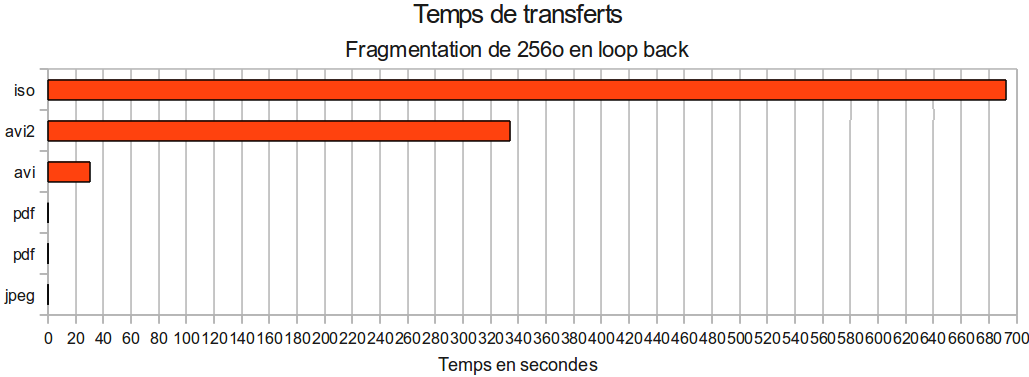
\includegraphics[scale=0.50]{t256loc.png}
\end{center}
\end{figure} 



\clearpage{}

\section{Variation de la taille des paquets}
\begin{figure}[!h]
\begin{center}
  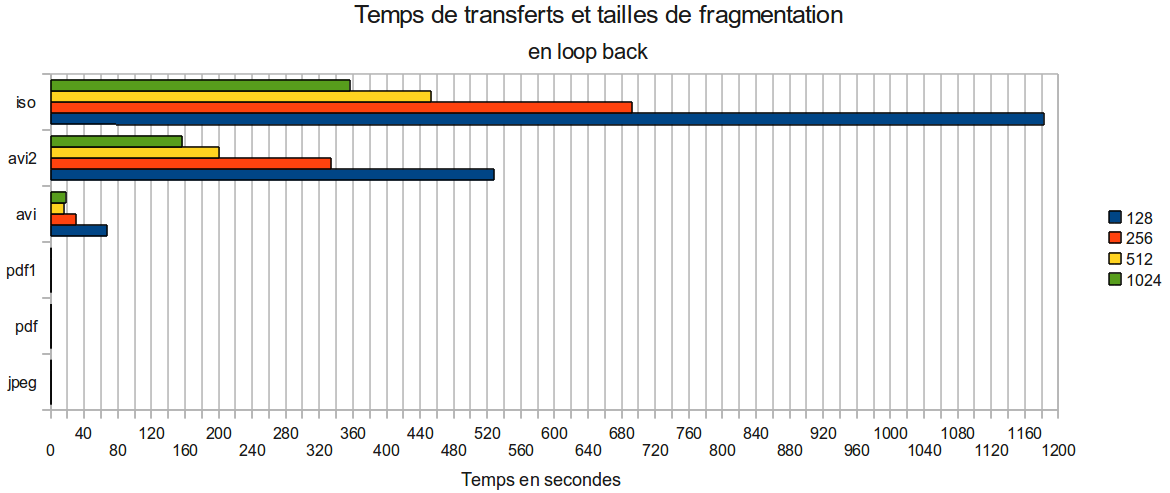
\includegraphics[scale=0.50]{tfragloc.png}
\end{center}
\end{figure} 
On constate que lors d'un transfert sur une même machine. L'augmentation de la taille de fragmentation permet une accélération de l'opération de transfert. Cependant pour une division supérieur à 1200 octets, des relevés de temps supplémentaires montre une stagnation des temps. Cela peut s'expliquer par le fait que le débit devient trop important pour les autres opérations (lectures/écriture dans le fichier ...). De la sorte, le temps minimum d'exécution est dépendant de ces opérations.

\clearpage{}



\section{Autres tests}
 blah blah blah blah blah blah blah blah blah blah blah blah blah blah blah blah blah blah blah blah blah blah blah blah blah blah blah blah blah blah blah blah

